\section{Architecture and Implementation} \label{sec:architecture}

\begin{figure}
	\centering
	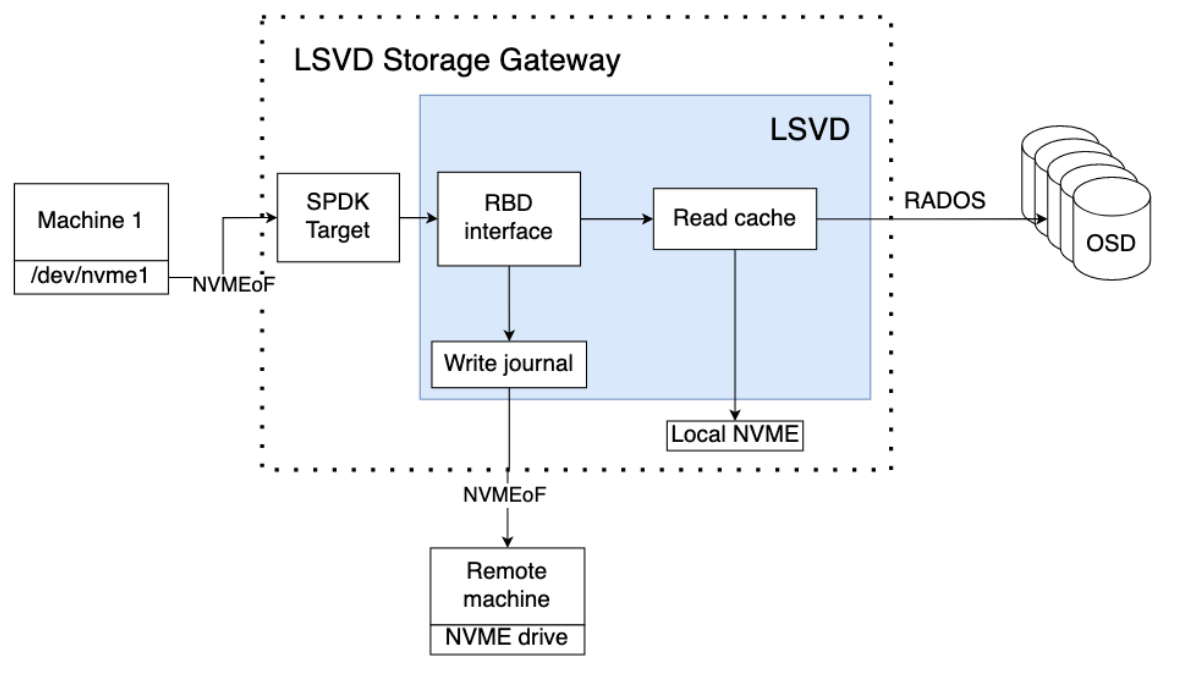
\includegraphics[width=1\linewidth]{figs/lsvd-highlv-arch.png}
	\caption[short]{TODO: High level architecture of Vinyl}
\end{figure}

The storage gateway is implemented as a new backend in SPDK, which exposes
Vinyl block devices as NVMe-oF or iSCSI devices to other clients. These are the
main components of the gateway: the \textit{write journal}, \textit{read cache},
\textit{LBA to object maps}, and \textit{garbage collector}.

Vinyl is implemented in roughly 15k lines of C++, and is publicly available on
Github at \redact{\url{https://github.com/CCI-MOC/lsvd-rbd}}. We currently use
Ceph RADOS as the object store backend, but the design is not tied to any
specific backend and can be easily ported to S3 compatible object stores.

\subsection{Gateway Server}

A key component of Vinyl is the intermediate gateway server, which sits between
the client and the backend storage.

Clients connect via NVMe-oF or iSCSI to the gateway, SPDK translates to Vinyl
commands. Vinyl, as a block storage device, support three major operations:
reading from a logical block address (LBA), writing to an LBA, and write
barriers that flush all outstanding writes to the backend. The gateway server
then translates these operations into the appropriate operations on the backend.

The choice \isaac{todo}

\subsection{Write Journal}

\begin{figure}
	\centering
	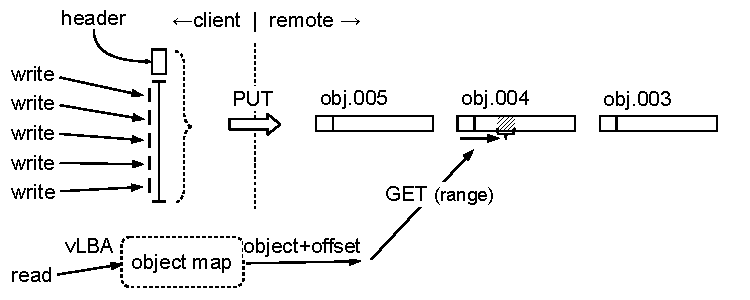
\includegraphics[width=1\linewidth]{figs/arch-translation.pdf}
	\caption[short]{TODO: Log structure}
\end{figure}

Log-structured storage systems treat the write log and the permanent data store
as one and the same. Writes are recorded on the log, and that's where it shall
stay until it's moved by a garbage collector or deleted.

Our design, however, does not allow for such a design. Our backend is an object
store, which usually uses immutable objects, and overwriting said object on
every client write would defeat the whole purpose of desiging the system for
high write efficiency. Instead, we separate out the write journal from the
backend, instead placing the write journal on a high-durability storage device
on a different failure domain than the gateway itself.

In practice, our write journal is a local NVMe drive on another server, and
writes are acknowledged only when they have been acklowledged by the NVMe.
Depending on the desired durability characteristings, it is possible to instead
store the write log on a remote server's RAM instead, which would introduce a
vulnerability to simultaneous failure of both the gateway and the remote write
log server. We present the performance tradeoffs of these two approaches in
Section~\ref{sec:evaluation}. If even more stringest guarantees are required of
the system, it is possible to use two remote write log servers instead of one.
\isaac{Probably cut this} The write log is also ideal use of persistent memory
technology with its characteristics of high longevity and latency, but due to
the discontinuation of Intel's Optane drives we did not pursue this approach.

The primary benefit of our log-structured approach is that it allows us to batch
many writes together into a single write to our backend, the object store. While
we still have to journal every single write received, we need not commit every
write to the backend before accumulating a sufficient amount (in this case,
8MiB) to overcome the costly nature of each backend write. It is true that we
increase the total write capacity amplification factor of the system by
double-writing each write, once to the journal and once to the backend, but we
reduce the amplification in terms of operations to the backend, and operations
overall.

The write journal in Vinyl is a ring buffer \isaac{but it isn't?}

\subsection{Clones and Snapshots}

As with other log-structured storage systems, we implement clones as a fork in
the log. \isaac{todo}

\subsection{Read cache}

Since backend objects are immutable, caching is much simpler without worrying
about entry invalidation or consistency. We dedicate much of the local NVMe
storage to a read cache of recently read objects, with simple CLOCK eviction.

The cache is shared between all clients, and thus is especially useful for cases
where many clients are reading the same data, such as booting a cluster of VMs
where their disk images were cloned from the same base image. This results in a
near 100\% cache hit rate for the booting VMs, greatly decreasing the burden on
both the backend and on cache space.

Entries in the cache are stored as fixed 64KiB blocks; reads are thus also
aligned to 64KiB boundaries. On a cache miss, a backend request is made for
cache-aligned 64KiB blocks, and the cache is populated with the returned data.
The major downside of this approach is the potential for major read
amplification in the event of many small reads that all miss and thrash the
cache, but in practice this is not a major issue as most read workloads exhibit
a high amount of locality and thus are well suited for caching. In the case
of radom small read workloads, we implement a cache bypass mode that triggers
when the read amplification rate rises above a threshold to prevent worst case
scenario amplification and cache thrashing.

On a flush to the backend, new objects are also directly inserted into the cache
to improve read-after-write performance. This also prevents consistency issues
around the newly-flushed request for reads that are issued when the backend
request is in-flight, as they will just hit the cache instead.

To improve performance in high-parellelism workloads, the cache is sharded into
16 shards, each of which may be backed by a separate NVMe or other storage
device. This means that in practice, for workloads with good locality, read
performance of Vinyl disks approaches that of the same disk backed by a local
SSD instead of a remote object store.

\subsection{VM Image Optimisations}

If the read workload is known ahead of time, as with VM image boots, we can also
re-organise the image to improve read performance. We do this by re-ordering the
image such that all reads are sequential in the space of the backend, if it's
not sequential in the LBA.

\timo{todo}
